\documentclass[12pt,a4paper]{report}
\synctex=1
\usepackage[utf8]{inputenc}
\usepackage[margin=1cm,bottom=2cm]{geometry}
\usepackage{graphicx}
%\usepackage{verbatim}
\usepackage{listings}
\usepackage{multicol}
\usepackage{libertine}
\usepackage{pgfornament}
\usepackage{eso-pic}
\usepackage{textcomp}
\usepackage{courier}
\usepackage[hangul]{kotex}
\linespread{1.3}

\title{
	\centering
	\pgfornament[width=12cm,color=teal]{84}\\
	\vspace{1cm}
	\fontsize{50}{50} \selectfont {동국 SW 공모대전\\SIC emulator 설명서}\\
	\pgfornament[width=12cm,color=teal]{88}\\
	\vfill}
\author{
	\LARGE
	\begin{tabular}{rl}
		\hline
		지도교수 : & 홍영식\\
		학번 : & 2016110056\\ 
		학과 : & 불교학부 \\
		이름 : & 박승원\\
		email : & zezeon@msn.com\\
		날짜 : & \today\\
		\hline
	\end{tabular}\vspace{2cm}
	\\
	\includegraphics[width=0.5\textwidth]{/home/zezeon/Dropbox/Photos/logo.jpg}
}
\date{}


\begin{document}
\maketitle

\tableofcontents

\noindent
\lstset{columns=flexible, tabsize=4, frame=single, showstringspaces=false, breaklines=true, upquote=true}

%\pagenumbering{gobble}
\lstset{language=C++}
\chapter{개발 목표}
\begin{itemize}
\item 현재 학교에서 SIC emulator로 쓰고 있는 프로그램은 윈도우에서 버추얼 박스 안에서 실행해야 하는 불편함이 있다.
\item 어느 시스템에서나 쓸 수 있게끔 텍스트 파일을 직접 에디트 하고 텍스트 파일로 결과를 받아볼 수 있는 간단한 SIC emulator가 더 편리할 것이다.
\item C나 C++로 짜서 어디서든 컴파일 할 수 있게 하고, 소오스를 스스로 고쳐보며 공부하는 것이 훨씬 나을 것이다.
\item 스스로의 공부를 위해서도 에뮬레이터를 만들어 보는 과정이 큰 공부가 될 것이다.
\end{itemize}
\chapter{소프트웨어 구성, 설명}
\section{SIC emulator에서의 Hello World 프로그램}
매크로 정의 부분은 매크로 전처리 기능을 보여주기 위해서 넣었다.
Hello World 기능과 아무 상관이 없다.
\lstinputlisting[caption={1.s : Hello World in SIC}]{1.s}
\lstinputlisting[caption={2.s : X 레지스터의 값을 1 증가시키는 모듈}]{2.s}
\paragraph{파일의 컴파일과 실행 절차}
\begin{enumerate}
	\item 전처리기(pre.x 1.s 1.s) : 1.s$\longrightarrow$1.s
	\item 컴파일(compile.x 1.s 1.o) : 1.s $\longrightarrow$ 1.o\quad 2.s $\longrightarrow$ 2.o
	\item 링킹(linker.x 1 2) : 1.o + 2.o $\longrightarrow$ 1.x
	\item 실행(run.x 1.x) : 1.x $\longrightarrow$ Hello World!
\end{enumerate}

1+2+3+4=통합 명령 : sic.x 1.s 2.s$\longrightarrow$Hello World!

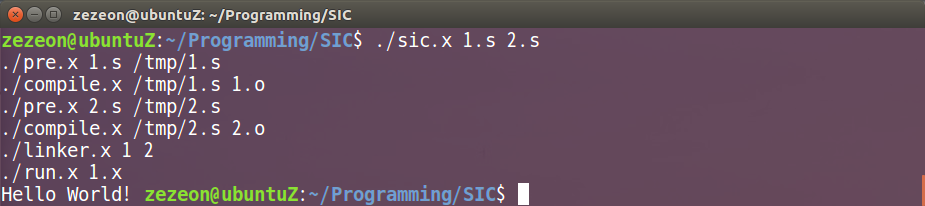
\includegraphics[width=\textwidth]{hello.png}
\section{Preprocessor}
\paragraph{source의 규칙}
\begin{itemize}
\item 소오스는 탭 혹은 공백 없이 시작하면 라벨이나 마크로 정의로 인식한다.
\item 탭 또는 공백이 연달아 오는 것은 하나의 공백으로 인식한다.
\item 세 번째 공백문자 이후는 모두 주석으로 인식한다. 
\item 대소문자는 구별하지 않는다.
\item SIC의 모든 명령어를 지원한다.(단, SIC/XE는 아님.)
\item 마크로 정의는 macro로 시작하고 mend로 끝난다.
\item 모듈파일은 반드시 프로그램의 시작 번지(start)보다 작은 숫자로 이름지어야 한다. 이 모듈은 jsub 2 이런 식으로 프로그램에서 호출할 수 있다.
\item 소오스의 모든 숫자는 십육진수로 인식한다.
\end{itemize}
\lstinputlisting[caption={1.s가 전처리된 소스 파일}]{/tmp/1.s}
macro가 치환되었고, byte c'Hello'가 byte + 16진수로 바뀌었다.
\lstinputlisting[caption={2.s가 전처리된 소스 파일}]{/tmp/2.s}
\section{Compiler}
\lstinputlisting[caption={1.o : 오브젝트 파일}]{1.o}
\paragraph{오브젝트 파일의 규칙}
\begin{itemize}
	\item 처음 세 줄은 시작번지, 데이터 시작 번지, 종료 번지이다.
	\item 다음부터는 주소와 기계어로 전처리된 소오스와 일대일 대응한다. 이 방식은 T 혹은 M 이후에 숫자를 주욱 나열하는 것보다 훨씬 가독성이 좋다.
	\item 0x1000번지를 보면 9042로 string,x의 X 레지스터 오프셋을 더하는 어드레스 지정방식이 적용된 것을 알 수 있다.
	\item jsub 2의 2는 링크 단계에서 주소를 찾아주게 된다.
\end{itemize}

\lstinputlisting[caption={2.o : 오브젝트 파일}]{2.o}
\section{Linker}
\lstinputlisting[caption={1.x : 1.o와 2.o가 링크된 실행 파일}]{1.x}
1015주소를 보면 48105f로 jsub 모듈의 주소가 치환되었다. 
2.o의 어드레스가 오프셋에 맞게 변환되었다.
\section{실행기(Interpreter)}
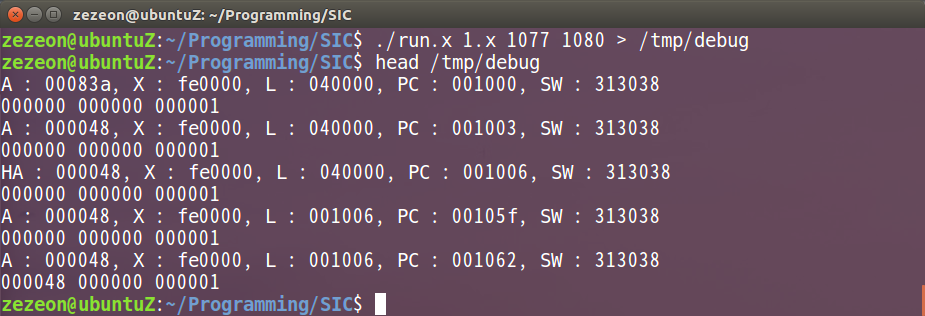
\includegraphics[width=\textwidth]{debug.png}

\paragraph{디버깅}
실행시 옵션을 주면 레지스터와 메모리의 특정 어드레스를 표현할 수 있다.

./run.x [실행화일] [표시할 시작어드레스] [표시할 종료어드레스]

의 형식이다.

컴파일 시에 에러가 발생하는 부분은 그 구문을 에러로 표시해준다.
\chapter{개발 효과}
\section{교육용 ADT로서의 소오스}
\lstinputlisting[caption={sic.h 헤더화일}]{sic.h}
\lstinputlisting[caption={sic.cc 구현화일}]{sic.cc}
교육과정상 C++을 먼저 배우고, 시스템 소프트웨어를 배우는데, C++을 이해하면 위의 헤더파일만 봐도 어느 정도 SIC의 작동원리를 이해할 수 있다.
하드웨어를 추상적으로 이해하는 데에 소오스 자체가 추상자료형을 제공하는 셈이다.
\section{SIC 에뮬레이터로서의 간편함}
\begin{itemize}
\item 커맨드 라인 환경이기에 어느 시스템에서나 호환성이 높다.
\item 이미 앞서서 오브젝트 파일에서 보았듯이, 기계어 코드가 매우 시인성이 높게 볼 수 있으며, 단순한 텍스트 파일이기 때문에, 얼다든지 직접 에디트하여 실행을 할 수도 있다.
\item 중간 처리 과정을 하나하나 분리하여 그 중간 결과물들을 텍스트로 볼 수 있다.
\item 소스를 직접 고쳐보며 배울 수 있다.
\end{itemize}
\end{document}
